%!tex program = lualatex
\documentclass[answers]{exam}
\usepackage{ctex}
\usepackage{graphicx}
\usepackage[margin=2cm]{geometry}
\usepackage{amsmath, amssymb}
\usepackage{csquotes}
\usepackage{tikz, pgfplots}
\usetikzlibrary{
	angles,
	backgrounds,
	calc,
	decorations.pathmorphing,
	decorations.pathreplacing,
	decorations.text,
	intersections,
	patterns,
	quotes,
	shapes,
	shapes.symbols,
}
\pagestyle{empty}
\newcounter{xcord}
\newcounter{ycord}
\newcounter{total}
\renewcommand{\labelenumi}{\textbf{\ifnum\value{enumi}<10 0\fi\arabic{enumi})}}

\pgfplotsset{compat=1.18}

\CorrectChoiceEmphasis{\color{blue!70!green}\bfseries}
\renewcommand{\solutiontitle}{\textbf{解:}}

\usepackage{array, tabularx}
\newcolumntype{C}{>{\centering\arraybackslash}X}
\newcolumntype{B}{>{\centering\bfseries\arraybackslash}X}
\catcode`\幺=0

\usepackage{tkz-euclide}

\begin{document}
\begin{center}
	\textbf{1997年普通高等学校招生考试(全国卷)}

	\textbf{\Large 理科数学}
\end{center}
\begin{questions}
	\question 设集合$M=\{x|0 \leqslant x < 2\}$,集合$N=\{x|x^2 - 2x - 3 <0\}$,集合$M\cap N=$ \hfill (\hspace{2cm})
	\begin{oneparchoices}
		\choice $\{x|0\leqslant x < 1\}$
		\CorrectChoice $\{x|0\leqslant x < 2\}$
		\choice $\{x|0\leqslant x \leqslant 1\}$
		\choice $\{x|0\leqslant x \leqslant 2\}$
	\end{oneparchoices}

	\begin{solution}
		集合$N=\{x|-1 < x < 3\}$,两个集合的范围如下图所示:

		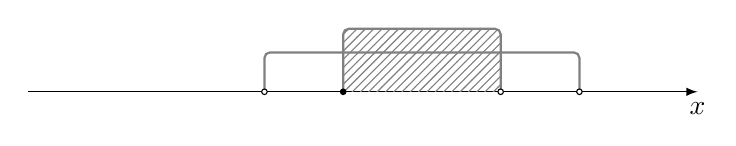
\begin{tikzpicture}
			\tkzInit[xmin=-4, xmax=4]
			\tkzDrawX

			\draw[rounded corners=2pt, thick, black!50] (-1,0) |- (3,.5) -- (3,0);
			\draw[black!50, thick, pattern=north east lines,pattern color=black!50, rounded corners=2pt] (0,0) |- (2,.8) -- (2,0);
			\draw [fill=white](-1,0) circle (1pt);
			\draw [fill=white](3,0) circle (1pt);
			\draw [fill=black](0,0) circle (1pt);
			\draw [fill=white](2,0) circle (1pt);
		\end{tikzpicture}
	\end{solution}

	\question 如果直线$ax+2y+2=0$与直线$3x-y-2=0$平行,那么系数$a=$ \hfs

	\begin{oneparchoices}
		\choice $-3$
		\CorrectChoice $-6$
		\choice $-\dfrac32$
		\choice $\dfrac23$
	\end{oneparchoices}

	\begin{solution}
		两条直线平行则其斜率相等,可得:
		\begin{equation*}
			-\frac{a}{2} = 3
		\end{equation*}
		所以答案为$a=-6$
	\end{solution}

\end{questions}
\end{document}
